\chapter{Minimizing Error Function with Gradient Descent}
Doing Deep Learning means training our models. These models are made up of parameters that are randomly initialized and gradually get closer to mapping our inputs to our outputs. This is done by minimizing our error function, and one of the key algorithms for minimizing error is the gradient descent algorithm. Once we are dealing with multilayer models, we need to find a way to backpropagate the changes, which we use the backpropagation algorithm for.


\section{Lesson Outline}
Improving our Machine Learning model means computing how far off our predictions are from their true values and minimizing the distance between those values. To do that, we'll need to understand how we can do that optimization programmatically. In this lesson, we will learn how to:

\begin{itemize}
    \item Create and manipulate PyTorch tensors
    \item Preprocess data using PyTorch
    \item Define and use loss functions to measure model performance
    \item Implement the foundational algorithms of deep learning: gradient descent and backpropagation
\end{itemize}
The skills we learn in this lesson will build the foundations needed for doing Deep Learning.

\section{PyTorch Basics}

\subsection{PyTorch and Tensors}

In the video, we covered a number of features of PyTorch. In general, it's a good idea to keep the \href{https://pytorch.org/docs/stable/index.html}{\textbf{PyTorch documentation}} handy. Most of what was demonstrated in this video are properties of \href{https://pytorch.org/docs/stable/tensors.html}{\textbf{Tensors}} or are parts of core \href{https://pytorch.org/docs/stable/torch.html}{\textbf{Torch}}.

Since PyTorch uses NumPy like indices, this \href{https://docs.scipy.org/doc/numpy-1.10.1/reference/arrays.indexing.html}{\textbf{SciPy documentation}} on indexing and slicing numpy arrays may be helpful.

\section{PreProcessing Data with PyTorch}
\href{https://www.youtube.com/watch?v=q8GER-HSg14&t=3s&ab_channel=Udacity}{Youtube} \newline

\subsection{Data Representation}

Rarely can we use "out of the box" input. We need our input to be tensors, but often our raw data consists of images, text, or tabular data, and we can't easily input those directly into our model.

\begin{itemize}
    \item For i\textbf{mage data}, we need the data to be turned into tensors with entries of the tensors as bit values in color channels (usually red, green, and blue).
    \item \textbf{Text data} needs to be tokenized, meaning, individual words or groups of letters need to be mapped to a token value.
    \item For \textbf{tabular data}, we have categorical values (high, medium, low, colors, demographic information, etc...) that we need to transform into numbers for processing.
\end{itemize}

\subsection{One-Hot Encoding}

Categorical values can become numbers. For instance, if you have three colors, Red, Blue, and Yellow, you can assign binary values representing if the color is present or not. The model can then easily compute how far two points are from each other, rather than simply assigning arbitrary values (like 1, 2, and 3 to the colors).

Note: One-Hot Encoding adds columns, which increases the dimensions of our tensors. If you have a lot of categorical features, this makes it even more complicated.

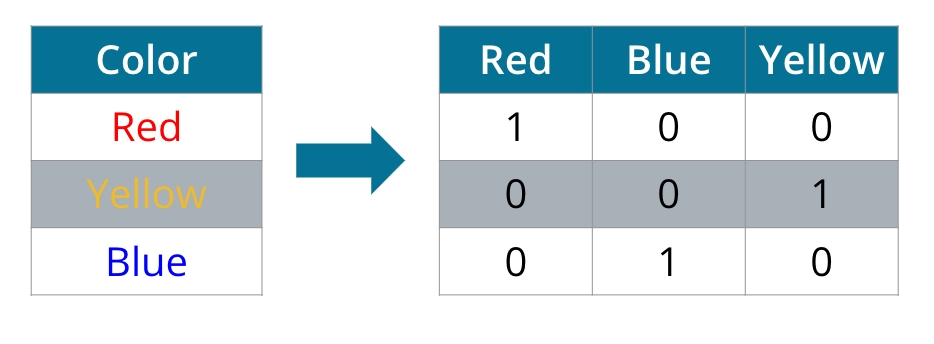
\includegraphics[width=1\linewidth]{img//intro/screen-shot-2022-06-27-at-11.16.07-am.jpeg}
\captionof{figure}{Example of One Hot Encoding}

One-hot encoding makes it easier to compute how away two points (with categorical data) are.

\subsection{Other preprocessing techniques}

Normalization maps numerical vlaues in a tensor to be between 0 and 1. It can help networks to train better.

Data preprocessing is also useful for data augmentation. It is especially useful to use preprocessing techniques to artificially increase the amount of training data that can be used. This is typically done by \textbf{flipping}, \textbf{cropping} images and \textbf{zooming} in on the images but retaining the label.

Label encoding, line one-hot encoding, can help us turn features that are words into features that are numbers. 

\subsection{Transforming Data for Neural Networks}

Often, we are faced with data that is not in a format conducive to use in neural networks in its raw form. Preprocessing is the act of turning data from that raw form into tensors that can be used as input to a neural network. This includes:

\begin{itemize}
    \item Encoding non-numerical features
    \item Converting images to tensors of bit values in color channels
    \item Tokenizing words
\end{itemize}

\section{Error Functions}
For the remainder of this lesson, we will be using \textit{error functions}. An \textbf{error function} is simply a function that measures how far the current state is from the solution. We can calculate the error and then make a change in an attempt to reduce the error—and then repeat this process until we have reduced the error to an acceptable level.


\section{Log-Loss Error Function}
A commonly-invoked metaphor is that the space of possible models is a mountain, and the ideal solution is at sea level. The specific model at any point in time is a location on the mountain. The error function in this metaphor is a means for measuring the altitude at that location. Iteratively improving the model means moving the model in a direction that reduces the altitude. IE, this means walking downhill or descending the gradient, hence “\textbf{gradient descent}”. \newline

Continuing the analogy, it is possible that some situations will result in the model ending up in a valley that is still above sea level, a “local minima.” This commonly occurs in machine learning. \newline

There are a few requirements for the error function in order for it to be used in gradient descent. The error function must be:

\begin{itemize}
    \item \textbf{Continuous}, and not discrete. The shape of the error function must be like a mountain and not like a staircase. With a discrete error function (such as a simple count of the number of misclassified points), a single small change may not have any detectable effect on the error.
    \item \textbf{Differentiable}.
\end{itemize}
A continuous error function implies that we also need continuous predictions. We'll do that in this lesson using the \textbf{log-loss} error function. Generally speaking, the log-loss function will assign a large penalty to incorrectly classified points and small penalties to correctly classified points. For a point that is misclassified, the penalty is roughly the distance from the boundary to the point. For a point that is correctly classified, the penalty is almost zero.\newline

We can then calculate a \textbf{total error} by adding all the errors from the corresponding points. Then we can use \textbf{gradient descent} to solve the problem, making very tiny changes to the parameters of the line in order to decrease the total error until we have reached an acceptable minimum.\newline

We need to cover some other concepts before we get into the specifics of how to calculate our log-loss function, but we'll come back to it when we dive into gradient descent later in the lesson.

\section{Maximum Likelihood}
\href{https://www.youtube.com/watch?v=1yJx-QtlvNI&t=5s&ab_channel=Udacity}{Youtube I}, \href{https://www.youtube.com/watch?v=6nUUeQ9AeUA&t=155s&ab_channel=Udacity}{Youtube II}\newline

Maximum likelihood is a method for choosing the best model given a set of labels. The best model is the one that gives the highest likelihood to the events that actually happened. In other words, we pick that model that gives the existing labels the highest probability. \newline

Consider an example where there are two models predicting the likelihood that a student gets accepted to a university. One predicts 80\% probability, the other, 55\%. If the student was accepted, then the model that predicted 80\% probability would be deemed the better model. \newline

The key idea is that we want to calculate \(P(all)\), which is the product of all the independent probabilities of \textit{each} point. This helps indicate how well the model performs in classifying all the points. To get the best model, we will want to maximize this probability. \newline

By this method, the model on the right in the image below would be the better model.

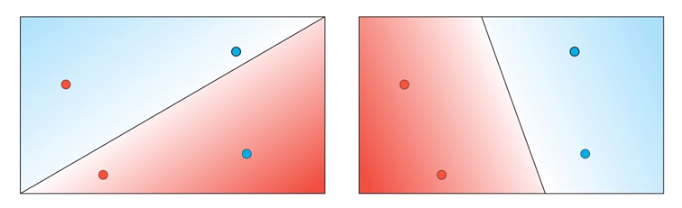
\includegraphics[width=1\linewidth]{img//intro/neural-networks-6.png}
 
We can also derive this result in a more analytically-rigorous fashion. Suppose that the probability of these points being blue is given by the values in the following image.

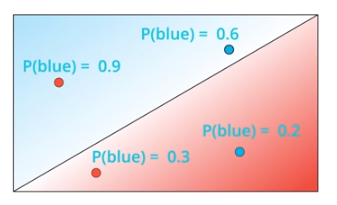
\includegraphics[width=0.5\linewidth]{img//intro/neural-networks-7.png}

We know that \(P(red) = 1 - P(blue)\), and we can calculate the probability that each of the four points are the color that they are: \(P(red) = 0.1\), \(P(blue) = 0.6\), \(P(red) 0.7\), and \(P(blue) = 0.2\). Assuming the colors are independent events, \(P(all)\) is the product of those individual probabilities.

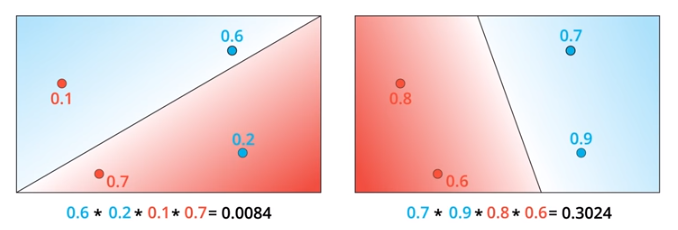
\includegraphics[width=1\linewidth]{img//intro/neural-networks-8.png}

High values of \(P(all)\) indicate the model classifies most points correctly with \(P(all)\) indicating how accurate the model is


\section{Cross Entropy}
\href{https://www.youtube.com/watch?v=LaYIdluNsZE&t=180s&ab_channel=Udacity}{Youtube}

\begin{itemize}
    \item The model estimates the probability distribution of the data.
    \item Model captures \textit{information} from the data in our parameters.
    \item Information is the representation of  the probability of an event in the unit of bits.
\end{itemize}
If we have an event X with probability p, the information provided by observing X is the negative logarithm of that probability \(I(X) = -log(p)\). \newline

If we have multiple events with multiple possible outcomes, we instead need to look at the entropy of the observations: \(H(X) = -E_{x \sim P}[log p(x)] = - \sum_i p_i log p_i\) \newline

If our data has some probability distribution and our model is trying to approximate that distribution, then our error is a function of the distance between these two probability distributions. How can we measure this distance? With Cross-Entropy.

\subsection{Measuring Distances between Distributions}

Cross-Entropy is a way of measuring the difference between two distributions. We define Cross-Entropy for binary labels and N examples as: \[-\sum_{i=1}^N y_i \log p_i + (1 - y_i)\log(1 - p_i) \]
Multi-Class Cross-Entropy is then defined for M labels and N examples as: \[-\sum_{i = 1}^N \sum_{j+1}^M y_{ij} \log p_{ij}\]
Cross-Entropy is one of the best ways to describe the difference between our predictions and the true labels.

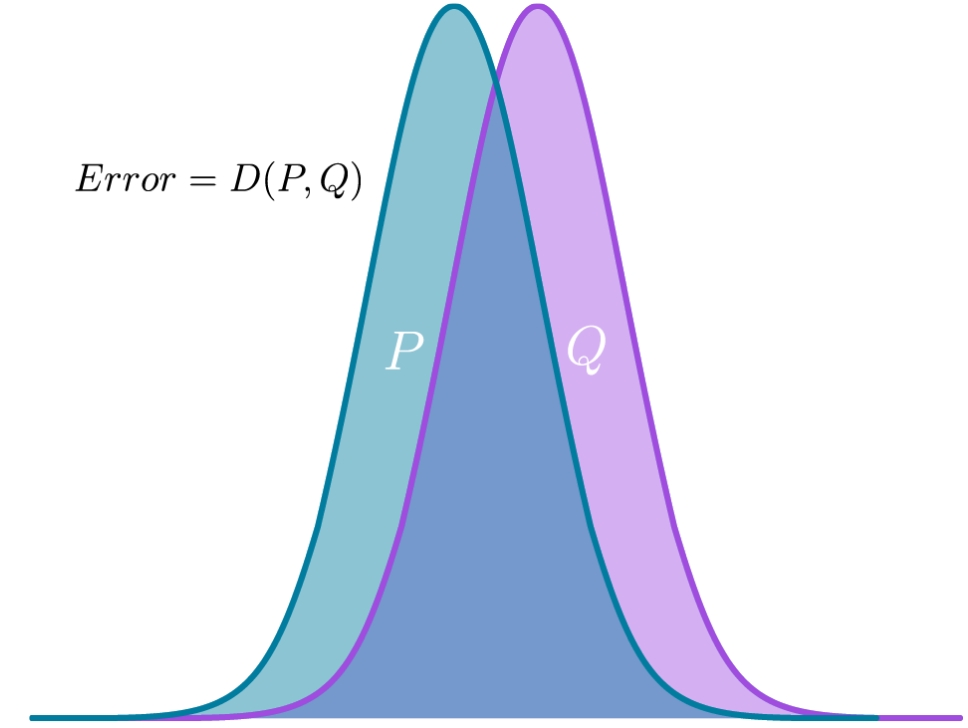
\includegraphics[width=0.75\linewidth]{img//intro/error.jpeg}

Minimizing cross-entropy is mathematically equivalent to maximizing log-likelihood.

\section{Gradient Descent}
\href{https://www.youtube.com/watch?v=rhVIF-nigrY&t=15s&ab_channel=Udacity}{Youtube}

In the last few sections, we learned that in order to minimize the error function, we need to take some derivatives. So let's get our hands dirty and actually compute the derivative of the error function. The first thing to notice is that the sigmoid function has a really nice derivative. Namely, \[\sigma'(x)=\sigma(x)(1-\sigma(x))\]
The reason for this is the following, we can calculate it using the quotient formula:
\[
\begin{split}
\sigma'(x) & = \frac{\partial}{\partial x} \frac{1}{1 + e^{-x}} \\
& = \frac{e^{-x}}{(1 + e^{-x})^2} \\
& = \frac{1}{1 + e^{-x}} \frac{e^{-x}}{1 + e^{-x}} \\
& = \sigma(x)(1-\sigma(x))
\end{split}
\]

And now, let's recall that if we have\(m\) points labelled \(x^{(1)}, x^{(2)}, ..., x^{(m)}\), the error formula is: \[E = -\frac{1}{m} \sum_{i=1}^m (y_i ln(\hat{y}_i) + (1 - y_i) ln(1 - \hat{y}_i))\]
where the prediction is given by \(\hat{y}_i = \sigma(Wx^{(x)} + b)\). \newline

Our goal is to calculate the gradient of \(E\), at a point \(x = (x_1, ..., x_n)\) given by the partial derivatives \[\nabla E = (\frac{\partial}{\partial w_1} E, …, \frac{\partial}{\partial w_n} E, \frac{\partial}{\partial b} E)\]

To simplify our calculations, we'll actually think of the error that each point produces, and calculate the derivative of this error. The total error, then, is the average of the errors at all the points. The error produced by each point is, simply,
\[E= -y ln(\hat{y}) - (1 - y) ln(1-\hat{y})\]

In order to calculate the derivative of this error with respect to the weights, we'll first calculate \(\frac{\partial}{\partial w_j} \hat{y}\). Recall that \(\hat{y}=\sigma(Wx+b)\), so:
\[
\begin{split}
    \frac{\partial}{\partial w_j} \hat{y} &= \frac{\partial}{\partial w_j} \sigma (Wx+b) \\
    &= \sigma{(Wx + b)}{(1 - \sigma(Wx +b))} \frac{\partial}{\partial w_j}{(Wx+b)} \\
    &= \hat{y} {(1-\hat{y})} \frac{\partial}{\partial w_j}{(Wx+b}\\
    &= \hat{y} {(1-\hat{y})} \frac{\partial}{\partial w_j} {(w_1 x_1 + ... + w_j x_j + ... + w_n x_n + b)} \\
    &= \hat{y} {(1-\hat{y})} x_j
\end{split}
\]

The last equality is because the only term in the sum which is not a constant with respect to \(w_j\) is precisely \(w_j x_j\), which clearly has derivative \(x_j\). \newline

Now, we can go ahead and calculate the derivative of the error \(E\) at a point \(x\), with respect to the weight \(w_j\).

\[
\begin{split}
    \frac{\partial}{\partial w_j} E &= \frac{\partial}{\partial w_j} {[-y \log(\hat{y}) - {(1-y)} \log(1 - \hat{y})]} \\
    &= -y \frac{\partial}{\partial w_j} \log(\hat{y}) - {(1 - y)} \frac{\partial}{\partial w_j} \log(1 - \hat{y}) \\
    &= -y \frac{1}{\hat{y}} \frac{\partial}{\partial w_j}\hat{y} - {(1 - y)} \frac{1}{1 - \hat{y}} \frac{\partial}{\partial w_j} (1 - \hat{y}) \\
    &= -y \frac{1}{\hat{y}} \hat{y} {(1 - \hat{y})}x_j - {(1 - y)} \frac{1}{1 - \hat{y}} {(-1)} \hat{y} {(1 - \hat{y})} x_j \\
    &= -y{(1 - \hat{y})} x_j + {(1 - y)} \hat{y}  x_j \\
    &= -{(y - \hat{y})}x_j
\end{split}
\]

A similar calculation will show us that \[\frac{\partial}{\partial b} E = -(y-\hat{y})\]

This actually tells us something very important. For a point with coordinates \((x_1, ..., x_n)\), label \(y\), and prediction \(\hat{y}\), the gradient of the error function at that point is \((- (y - \hat{y})x_1, ..., (y - \hat{y})x_n, (y - \hat{y}))\). In summary, the gradient is \[\nabla E = -(y-\hat{y})(x_1,…,x_n,1)\]
This means the gradient is a scalar times the coordinates of the point, and that scalar is a multiple of the difference between the label and the prediction. This means that:

\begin{itemize}
    \item the \textbf{closer the label is to the prediction}, the smaller the gradient, and
    \item the \textbf{farther the label is from the prediction}, the larger the gradient.
\end{itemize}
Therefore:

\begin{itemize}
    \item If a point is \textbf{well classified}, we will get a \textbf{small gradient}.
    \item If it’s \textbf{poorly classified}, the \textbf{gradient will be large}.
\end{itemize}
So, a small gradient means we'll change our coordinates by a little bit, and a large gradient means we'll change our coordinates by a lot.

If this sounds anything like the perceptron algorithm, this is no coincidence! We'll see it in a bit.
\subsection{Gradient Descent Step}

Therefore, since the gradient descent step simply consists in subtracting a multiple of the gradient of the error function at every point, then this updates the weights in the following way: \[w'_i \leftarrow w_i - \alpha[-(y-\hat{y})x_i]\]
which is equivalent to \[w'_i \leftarrow w_i + \alpha(y+\hat{y})x_i\]
Similarly, it updates the bias in the following way: \[b'_i \leftarrow b_i + \alpha(y+\hat{y})x_i\]
\textit{Note:} Since we've taken the average of the errors, the term we are adding should be \(\frac{1}{m} \alpha\) instead of \(\alpha\), but as \(\alpha\) is a constant, then in order to simplify calculations, we'll just take \(\frac{1}{m}\alpha\) to be our learning rate, and abuse the notation by just calling it \(\alpha\).

\section{Logistic Regression}

Now, we're finally ready for one of the most popular and useful algorithms in machine learning, and the building block of all that constitutes deep learning: The \textbf{logistic regression} algorithm. And it basically goes like this:

\begin{itemize}
    \item Take your data
    \item Pick a random model
    \item Calculate the error
    \item Minimize the error, and obtain a better model
    \item Enjoy!
\end{itemize}

\subsection{Calculating the Error Function}
\href{https://www.youtube.com/watch?v=V5kkHldUlVU&t=2s&ab_channel=Udacity}{Youtube} \newline

\subsubsection{Binary Classification}
\[Error\ Function = - \frac{1}{m} \sum_{i=1}^m (1-y_i)(ln(1-\hat{y}_i)) + y_iln(\hat{y_i})\]
Since \(\hat{y} = \sigma(Wx+b)\), we can substitute as follows: \[E(W,b) = - \frac{1}{m} \sum_{i=1}^m (1-y_i)(ln(1-\sigma(Wx^{(i)}+b))) + y_iln(\sigma(Wx^{(i)}+b))\]

In that formula, \(y_i\) is the label of the point  \(x^{(i)}\).

\subsubsection{Multi-Class Classification}
\[Error\ Function = -\frac{1}{m} \sum_{i=1}^m \sum_{j=1}^n y_{ij} ln(\hat{y_{ij}})\]

Now that we know how to calculate the error, our goal will be to minimize it.

\subsection{Minimizing the Error Function}
\href{https://www.youtube.com/watch?v=KayqiYijlzc&t=1s&ab_channel=Udacity}{Youtube} \newline

We begin with random weights, \(\sigma(Wx+b)\), which has a corresponding error function, \(E(W,b)\) given by the formula in the section above. The goal when minimizing the error function is to descend the gradient function. This is accomplished by moving the classification line until we arrive at a configuration with lower error. The separating line is given by \(\sigma(W’x+b')\) and the error is given by \(E(W',b')\).

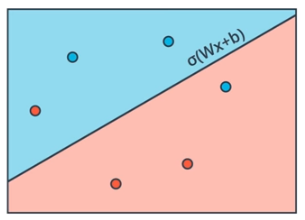
\includegraphics[width=0.5\linewidth]{img//intro//neural-networks-18.png}
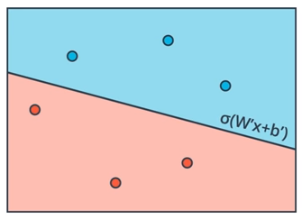
\includegraphics[width=0.5\linewidth]{img//intro//neural-networks-19.png}

This is accomplished with the gradient descent algorithm.


\section{Exercise: Implementing Gradient Descent}

Okay, now we know how to update our weights:

\[\Delta w_{ij} = \eta \cdot \delta_j \cdot x_i\]


You've seen how to implement that for a single update, but how do we translate that code to calculate many weight updates so our network will learn? \newline

As an example, I'm going to have you use gradient descent to train a network on graduate school admissions data (found at \href{https://stats.idre.ucla.edu/stat/data/binary.csv}{\textbf{http://www.ats.ucla.edu/stat/data/binary.csv}}). This dataset has three input features: GRE score, GPA, and the rank of the undergraduate school (numbered 1 through 4). Institutions with rank 1 have the highest prestige, those with rank 4 have the lowest.

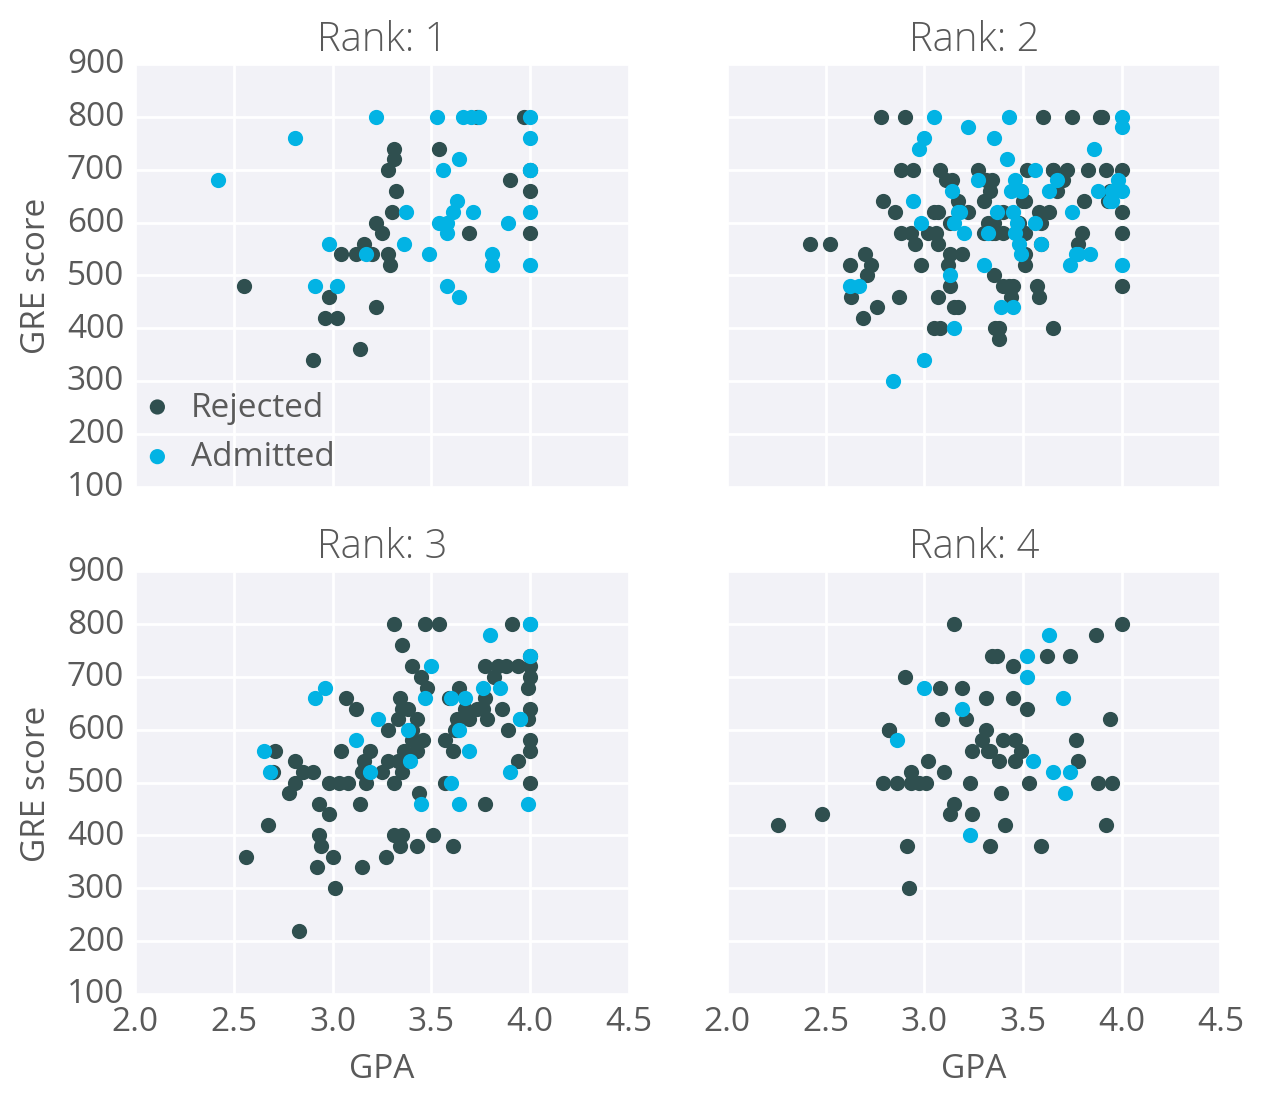
\includegraphics[width=1\linewidth]{img//intro/admissions-data.png}

The goal here is to predict if a student will be admitted to a graduate program based on these features. For this, we'll use a network with one output layer with one unit. We'll use a sigmoid function for the output unit activation.

\subsection{Data cleanup}

You might think there will be three input units, but we actually need to transform the data first.

\begin{itemize}
    \item The \verb|rank| feature is categorical, the numbers don't encode any sort of relative values.
    \item Rank 2 is not twice as much as rank 1, rank 3 is not 1.5 more than rank 2.
    \item Instead, we need to use \href{https://en.wikipedia.org/wiki/Dummy_variable_(statistics)}{\textbf{dummy variables}} to encode \verb|rank|, splitting the data into four new columns encoded with ones or zeros.
    \item Rows with rank 1 have one in the rank 1 dummy column, and zeros in all other columns.
    \item Rows with rank 2 have one in the rank 2 dummy column, and zeros in all other columns. And so on.
\end{itemize}

\subsubsection{Standardizing the GRE and GPA Data}

We'll also need to standardize the GRE and GPA data, which means scaling the values such that they have zero mean and a standard deviation of 1.

\begin{itemize}
    \item This is necessary because the sigmoid function squashes really small and really large inputs.
    \item The gradient of really small and large inputs is zero, which means that the gradient descent step will go to zero too.
    \item Since the GRE and GPA values are fairly large, we have to be really careful about how we initialize the weights or the gradient descent steps will die off and the network won't train.
    \item Instead, if we standardize the data, we can initialize the weights easily and everyone is happy.
\end{itemize}
This is just a brief run-through, you'll learn more about preparing data later. If you're interested in how I did this, check out the \verb|data_prep.py| file in the programming exercise below.

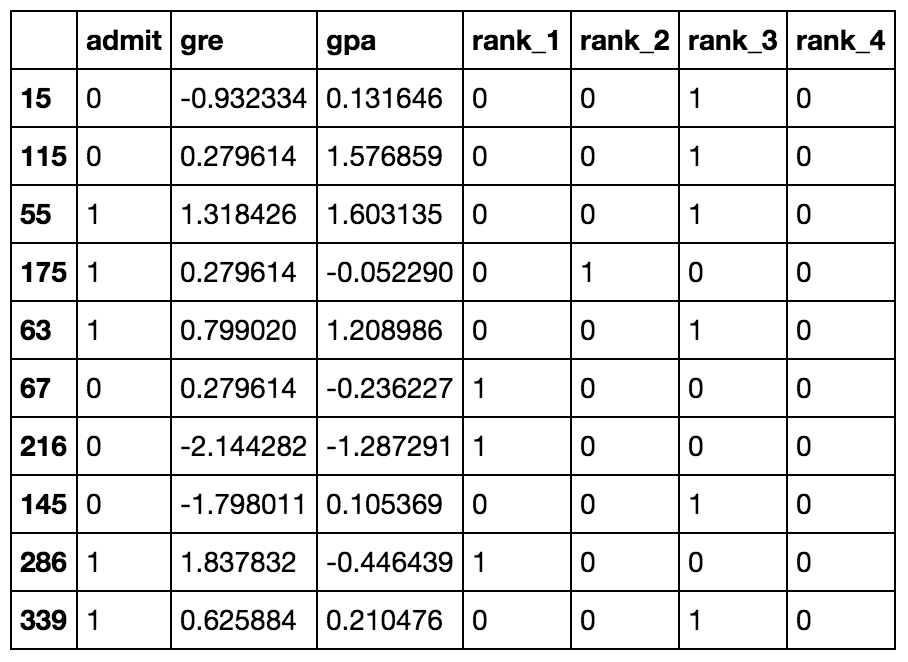
\includegraphics[width=1\linewidth]{img//intro/example-data.png}
\captionof{figure}{Ten rows of the data after transformations.}


\subsubsection{Mean Square Error}

We're going to make a small change to how we calculate the error here. Instead of the SSE, we're going to use the \textbf{mean} of the square errors (MSE). Now that we're using a lot of data, summing up all the weight steps can lead to really large updates that make the gradient descent diverge. To compensate for this, you'd need to use a quite small learning rate. Instead, we can just divide by the number of records in our data, \(m\) to take the average. This way, no matter how much data we use, our learning rates will typically be in the range of 0.01 to 0.001. Then, we can use the MSE (shown below) to calculate the gradient and the result is the same as before, just averaged instead of summed.
\[E=\frac{1}{2m}\sum_{\mu}(y^{\mu}-\hat{y}^{\mu})^2\]
Here's the general algorithm for updating the weights with gradient descent:

\begin{itemize}
    \item Set the weight step to zero: \(\Delta w_i = 0\)
    \item For each record in the training data:

\begin{itemize}
        \item Make a forward pass through the network, calculating the output \(\hat{y}=f(\sum_i w_i x_i)\)
        \item Calculate the error term for the output unit, \(\delta=(y-\hat{y})\cdot f'(\sum_i w_i x_i)\)
        \item Update the weight step \(\Delta w_i=\Delta w_i + \delta x_i\)
\end{itemize}

    \item Update the weights \(w_i=w_i+\eta \Delta w_i/m\) where \(\eta\) is the learning rate and \(m\) is the number of records. Here we're averaging the weight steps to help reduce any large variations in the training data.
    \item Repeat for \(e\) epochs.
\end{itemize}
You can also update the weights on each record instead of averaging the weight steps after going through all the records. \newline

Remember that we're using the sigmoid for the activation function, \[f(h)=\frac{1}{1+e^{-h}}\]

And the gradient of the sigmoid is \[f'(h)=f(h)(1-f(h))\]

where \(h\) is the input to the output unit,\[h=\sum_i w_i x_i\]

\subsection{Implementing with NumPy}

For the most part, this is pretty straightforward with NumPy.

First, you'll need to initialize the weights. We want these to be small such that the input to the sigmoid is in the linear region near 0 and not squashed at the high and low ends. It's also important to initialize them randomly so that they all have different starting values and diverge, breaking symmetry. So, we'll initialize the weights from a normal distribution centered at 0. A good value for the scale is \(\frac{1}{n}\)  where \(n\) is the number of input units. This keeps the input to the sigmoid low for increasing numbers of input units.

\begin{lstlisting}
weights = np.random.normal(scale=1/n_features**.5, size=n_features)
\end{lstlisting}

NumPy provides a function \lstinline|np.dot()| that calculates the dot product of two arrays, which conveniently calculates\textit{h} for us. The dot product multiplies two arrays element-wise, the first element in array 1 is multiplied by the first element in array 2, and so on. Then, each product is summed.

\begin{lstlisting}
## input to the output layer
output_in = np.dot(weights, inputs)
\end{lstlisting}

And finally, we can update \(\Delta w_i\) and \(w_i\) by incrementing them with \lstinline|weights += ...| which is shorthand for \lstinline|weights = weights + ...|.


\subsubsection{Efficiency tip!}

You can save some calculations since we're using a sigmoid here. For the sigmoid function, \(f'(h)=f(h)(1-f(h))\). That means that once you calculate \(f(h)\), the activation of the output unit, you can use it to calculate the gradient for the error gradient.

\subsubsection{Programming exercise}

Below, you'll implement gradient descent and train the network on the admissions data. Your goal here is to train the network until you reach a minimum in the mean square error (MSE) on the training set. You need to implement:

\begin{itemize}
    \item The network output: \lstinline|output|.
    \item The output error: \lstinline|error|.
    \item The error term: \lstinline{error_term}.
    \item Update the weight step: \lstinline{del_w +=}.
    \item Update the weights: \lstinline|weights +=|.
\end{itemize}
After you've written these parts, run the training by pressing Shift + Enter on the cell containing the code. The MSE will print out, as well as the accuracy on a test set, the fraction of correctly predicted admissions.

Feel free to play with the hyperparameters and see how it changes the MSE.

\begin{lstlisting}
import numpy as np
from data_prep import features, targets, features_test, targets_test

def sigmoid(x):
    """
    Calculate sigmoid
    """
    return 1 / (1 + np.exp(-x))

def update_weights(weights, features, targets, learnrate):
    """
    Complete a single epoch of gradient descent and return updated weights
    """
    del_w = np.zeros(weights.shape)
    # Loop through all records, x is the input, y is the target
    for x, y in zip(features.values, targets):
        # TODO: Calculate the output of f(h) by passing h (the dot product
        # of x and weights) into the activation function (sigmoid).
        # Replace None with appropriate code
        output = sigmoid(np.dot(x, weights))

        # TODO: Calculate the error by subtracting the network output
        # from the target (y).
        # Replace None with appropriate code
        error = y - output

        # TODO: Calculate the error term by multiplying the error by the
        # gradient. Recall that the gradient of the sigmoid f(h) is
        # f(h)*(1-f(h)) so you do not need to call any additional
        # functions and can simply apply this formula to the output and
        # error you already calculated.
        # Replace None with appropriate code
        error_term = error * output * (1 - output)

        # TODO: Update the weight step by multiplying the error term by
        # the input (x) and adding this to the current weight step.
        # Replace 0 with appropriate code
        del_w += error_term * x

    n_records = features.shape[0]
    # TODO: Update the weights by adding the learning rate times the
    # change in weights divided by the number of records.
    # Replace 0 with appropriate code
    weights += learnrate * del_w / n_records
    
    return weights

def gradient_descent(features, targets, epochs=1000, learnrate=0.5):
    """
    Perform the complete gradient descent process on a given dataset
    """
    # Use to same seed to make debugging easier
    np.random.seed(42)
    
    # Initialize loss and weights
    last_loss = None
    n_features = features.shape[1]
    weights = np.random.normal(scale=1/n_features**.5, size=n_features)

    # Repeatedly update the weights based on the number of epochs
    for e in range(epochs):
        weights = update_weights(weights, features, targets, learnrate)

        # Printing out the MSE on the training set every 10 epochs.
        # Initially this will print the same loss every time. When all of
        # the TODOs are complete, the MSE should decrease with each
        # printout
        if e % (epochs / 10) == 0:
            out = sigmoid(np.dot(features, weights))
            loss = np.mean((out - targets) ** 2)
            if last_loss and last_loss < loss:
                print("Train loss: ", loss, "  WARNING - Loss Increasing")
            else:
                print("Train loss: ", loss)
            last_loss = loss
            
    return weights

# Calculate accuracy on test data
weights = gradient_descent(features, targets)
tes_out = sigmoid(np.dot(features_test, weights))
predictions = tes_out > 0.5
accuracy = np.mean(predictions == targets_test)
print("Prediction accuracy: {:.3f}".format(accuracy))
\end{lstlisting}

\section{Perceptron}
\href{https://www.youtube.com/watch?v=O3JyyRSMHAQ&t=72s&ab_channel=Udacity}{Youtube}\newline

A perceptron is the building block of neural networks, and it's an encoding of our equation into a small graph. The perceptron receives the points as inputs, like in the image below, and returns \(1\) if the point is in the positive area, and a \(0\) otherwise.

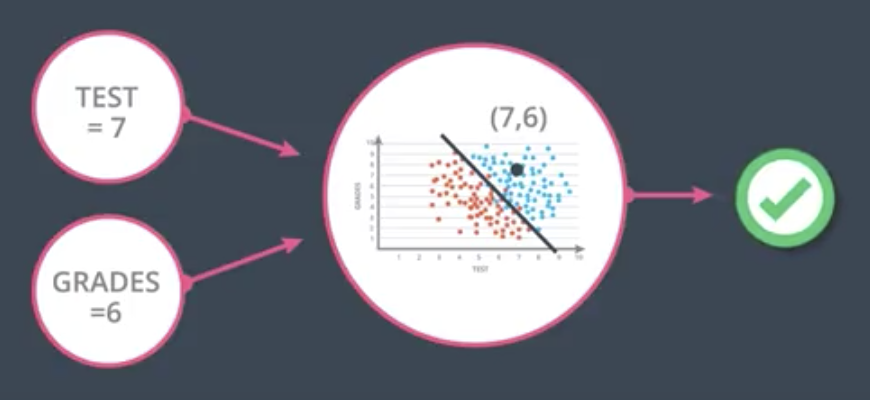
\includegraphics[width=1\linewidth]{img//intro/perceptron-4.png}

Recall that our equation is score equals \( (2 \cdot test) + (1 \cdot grade) - 18\) and our prediction consists of accepting the student if the score is positive or zero and rejecting them if the score is negative. \newline

The weights 2, 1, and -18, are what define the linear equation and will be used as labels in the graph. The 2 and the 1 will label the edges coming from \(x_1\) and \(x_2\) respectively, and the bias unit -18 will label the node.
\textit{Thus, when we see a node with these labels, we can think of the linear equation they generate.} \newline

The bias can be thought of as another input with magnitude 1 and edges with weights equal to the bias term, as show below.

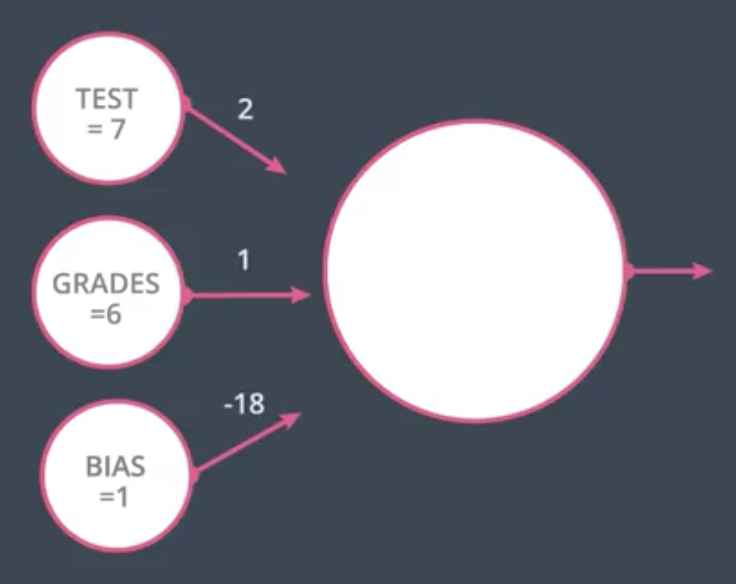
\includegraphics[width=1\linewidth]{img//intro/perceptron-5.png}

In the case of the example above:
\[Score = 2 \cdot 7 + 1 \cdot 6 - 18 \cdot 1 = 2\]
Since \(2 \geq 0\), the perceptron would output \(1\). \newline

In the general case, a node will have inputs coming in with values \(X_1\) up to \(X_n\) and 1, and edges with weights \(W_1\) up to \(W_n\), and \(b\) corresponding to the bias unit. The node calculates the linear equation
\[Wx + b = \sum^n_{i = 1} W_i X_i + b\]
This node then checks if the value is zero or greater, and if it is the node returns a value of one for yes. If not, the node returns a value of zero for no. \newline

\section{Multilayer Perceptrons}

Adding a “hidden” layer of perceptrons allows the model to find solutions to linearly inseparable problems. An example of this architecture is shown below.

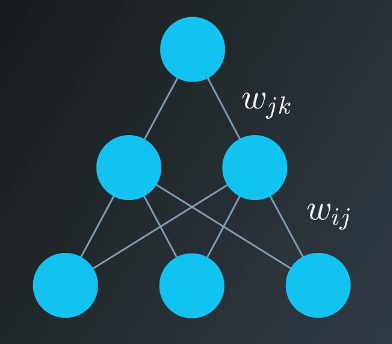
\includegraphics[width=0.5\linewidth]{img//intro//multilayer-perceptrons-1.png}

3 input layers, 1 output layers and 2 middle layers. These middle layers are called \textbf{hidden layers}.

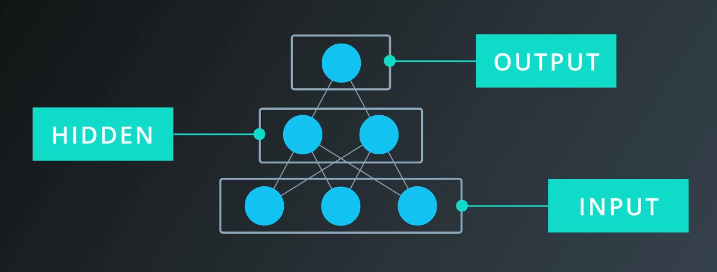
\includegraphics[width=0.5\linewidth]{img//intro//multilayer-perceptrons-2.png}

The input to the hidden layer is the same as it was before, as is the the activation function.

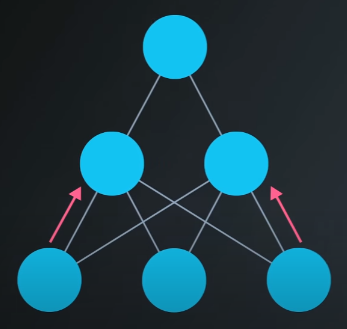
\includegraphics[width=0.5\linewidth]{img//intro//multilayer-perceptrons-3.png}

\[h_j = \sum_i w_{ij} \cdot x_i + b_j\]
\[a_j = sigmoid(h_j)\]

The input to the output layer is the output of the hidden layer.

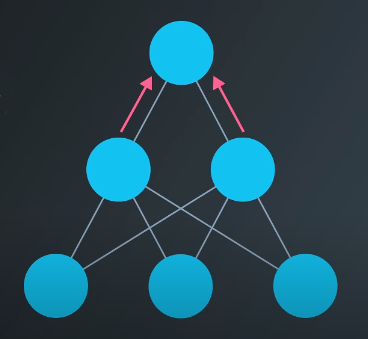
\includegraphics[width=0.5\linewidth]{img//intro//multilayer-perceptrons-4.png}

\[o_k = \sum_j w_{jk} \cdot a_j + b_j\]
\[a_k = sigmoid(o_k)\]

Stacking more and more layers helps the network learn more patterns. This is where the term “deep learning” comes from.

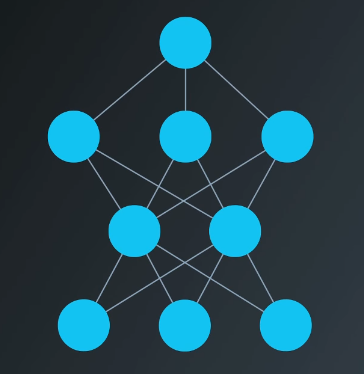
\includegraphics[width=0.5\linewidth]{img//intro//multilayer-perceptrons-5.png}

\subsection{Implementing the hidden layer}

\subsubsection{Prerequisites}
Below, we are going to walk through the math of neural networks in a multilayer perceptron. With multiple perceptrons, we are going to move to using vectors and matrices. To brush up, be sure to view the following:

\begin{enumerate}
    \item Khan Academy's \href{https://www.khanacademy.org/math/linear-algebra/vectors-and-spaces/vectors/v/vector-introduction-linear-algebra}{\textbf{introduction to vectors}}.
    \item Khan Academy's \href{https://www.khanacademy.org/math/precalculus/x9e81a4f98389efdf:matrices}{\textbf{introduction to matrices}}.
\end{enumerate}

\subsubsection{Derivation}
Before, we were dealing with only one output node which made the code straightforward. However now that we have multiple input units and multiple hidden units, the weights between them will require two indices: \(w_{ij}\) where \(i\) denotes input units and \(j\) are the hidden units. \newline

For example, the following image shows our network, with its input units labeled \(x_1, x_2,\) and \(x_3\), and its hidden nodes labeled \(h_1\) and \(h_2\):

 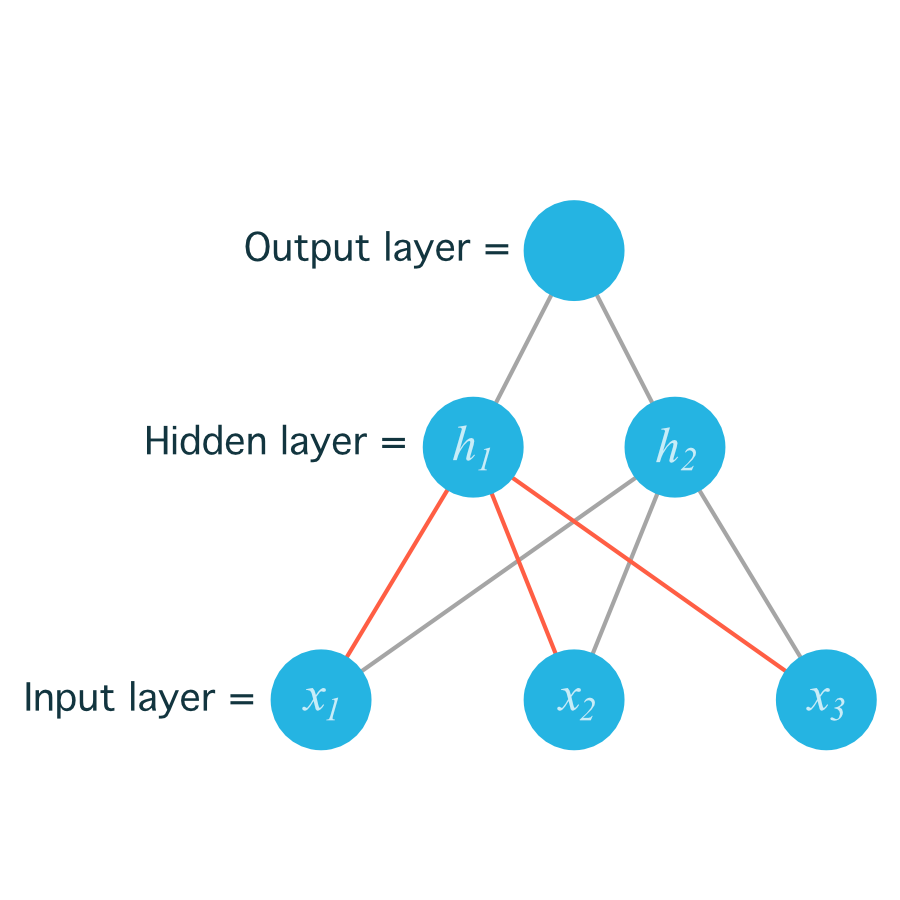
\includegraphics[width=0.5\linewidth]{img//intro//network-with-labeled-nodes.png}

The lines indicating the weights leading to \(h_1\) have been colored differently from those leading to \(h_2\) just to make it easier to read. \newline

Now to index the weights, we take the input unit number for the \(_i\) and the hidden unit number for the \(_j\). That gives us
\begin{itemize}
    \item \(w_{11}\) for the weight leading from \(x_1\) to \(h_1\), and
    \item \(w_{12}\) for the weight leading  from \(x_1\) to \(h_2\).
\end{itemize}

The following image includes all of the weights between the input layer and the hidden layer, labeled with their appropriate \(w_{ij}\) indices:

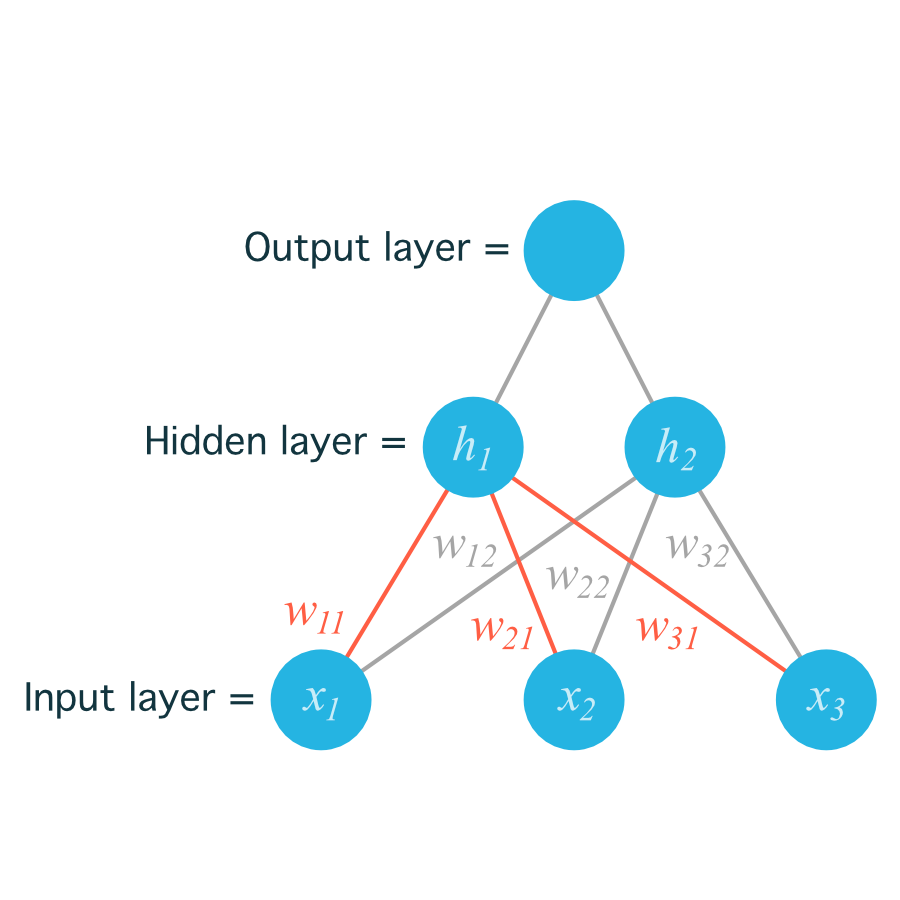
\includegraphics[width=0.5\linewidth]{img//intro//network-with-labeled-weights.png}

Before, we were able to write the weights as an array, indexed as \(w_i\). \newline

But now, the weights need to be stored in a \textbf{matrix}, indexed as \(w_{ij}\). Each \textbf{row} in the matrix will correspond to the weights \textbf{leading out} of a \textbf{single input unit}, and each \textbf{column} will correspond to the weights \textbf{leading in} to a \textbf{single hidden unit}. For our three input units and two hidden units, the weights matrix looks like this:

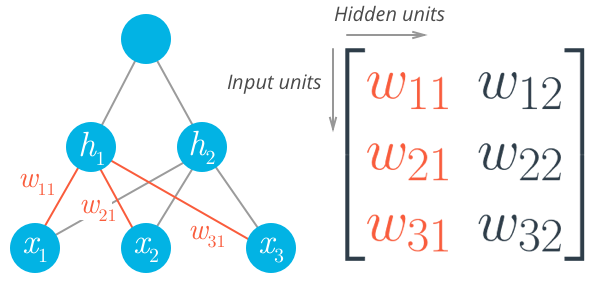
\includegraphics[width=0.5\linewidth]{img//intro//multilayer-diagram-weights.png}
\captionof{figure}{Weights matrix for 3 input units and 2 hidden units}

Be sure to compare the matrix above with the diagram shown before it so you can see where the different weights in the network end up in the matrix.

To initialize these weights in NumPy, we have to provide the shape of the matrix. If \lstinline{features} is a 2D array containing the input data:

\begin{lstlisting}
## Number of records and input units
n_records, n_inputs = features.shape
## Number of hidden units
n_hidden = 2
weights_input_to_hidden = np.random.normal(0, n_inputs**-0.5, size=(n_inputs, n_hidden))
\end{lstlisting}

This creates a 2D array (i.e. a matrix) named \verb|weights_input_to_hidden| with dimensions \verb|n_inputs| by \verb|n_hidden|. Remember how the input to a hidden unit is the sum of all the inputs multiplied by the hidden unit's weights. So for each hidden layer unit, \(h_{ij}\), we need to calculate the following: \[h_j = \sum_i w_{ij} x_i\]

To do that, we now need to use \href{https://en.wikipedia.org/wiki/Matrix_multiplication}{\textbf{matrix multiplication}}. If your linear algebra is rusty, I suggest taking a look at the suggested resources in the prerequisites section. For this part though, you'll only need to know how to multiply a matrix with a vector. \newline

In this case, we're multiplying the inputs (a row vector here) by the weights. To do this, you take the dot (inner) product of the inputs with each column in the weights matrix. For example, to calculate the input to the first hidden unit, \(j = 1\), you'd take the dot product of the inputs with the first column of the weights matrix, like so:

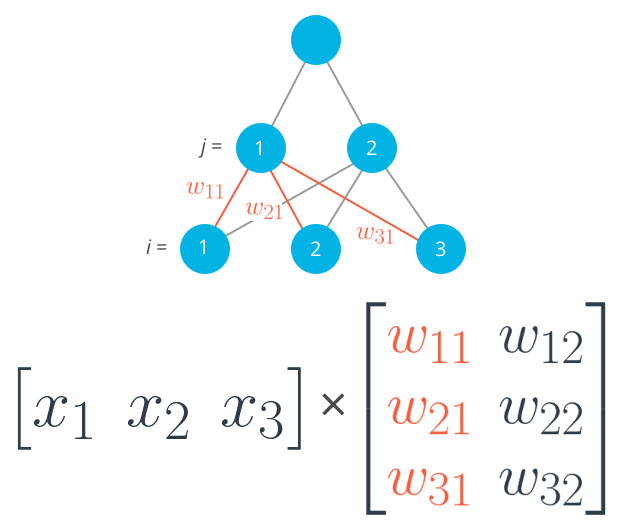
\includegraphics[width=0.75\linewidth]{img//intro//input-times-weights.png}
\captionof{figure}{Calculating the input to the first hidden unit with the first column of the weights matrix.}

\[h_1 = x_1 w_{11} + x_2 w_{21} + x_3 w_{31}\]

And for the second hidden layer input, you calculate the dot product of the inputs with the second column. And so on and so forth. \newline

In NumPy, you can do this for all the inputs and all the outputs at once using \lstinline{np.dot}

\begin{lstlisting}
hidden_inputs = np.dot(inputs, weights_input_to_hidden)
\end{lstlisting}

You could also define your weights matrix such that it has dimensions \lstinline{n_hidden} by \lstinline{n_inputs} then multiply like so where the inputs form a column vector:

\[h_j =
\begin{bmatrix}
w_{11} & w_{12} & w_{13} \\
w_{21} & w_{22} & w_{23}
\end{bmatrix}
\times
\begin{bmatrix}
x_1 \\
x_2 \\
x_3
\end{bmatrix}
\]

\textbf{Note}: The weight indices have changed in the above image and no longer match up with the labels used in the earlier diagrams. That's because, in matrix notation, the row index always precedes the column index, so it would be misleading to label them the way we did in the neural net diagram. Just keep in mind that this is the same weight matrix as before, but rotated so the first column is now the first row, and the second column is now the second row. If we were to use the labels from the earlier diagram, the weights would fit into the matrix in the following locations:

\[
\begin{bmatrix}
w_{11} & w_{21} & w_{31} \\
w_{12} & w_{22} & w_{32}
\end{bmatrix}
\]
\captionof{figure}{Weight matrix shown with labels matching earlier diagrams.}

Remember, the above is \textbf{not} a correct view of the \textbf{indices}, but it uses the labels from the earlier neural net diagrams to show you where each weight ends up in the matrix. \newline

The important thing with matrix multiplication is that \textit{the dimensions match}. For matrix multiplication to work, there has to be the same number of elements in the dot products. In the first example, there are three columns in the input vector, and three rows in the weights matrix. In the second example, there are three columns in the weights matrix and three rows in the input vector. If the dimensions don't match, you'll get this:

\begin{lstlisting}
## Same weights and features as above, but swapped the order
hidden_inputs = np.dot(weights_input_to_hidden, features)
---------------------------------------------------------------------------
ValueError                                Traceback (most recent call last)
<ipython-input-11-1bfa0f615c45> in <module>()
----> 1 hidden_in = np.dot(weights_input_to_hidden, X)

ValueError: shapes (3,2) and (3,) not aligned: 2 (dim 1) != 3 (dim 0)
\end{lstlisting}

The dot product can't be computed for a 3x2 matrix and 3-element array. That's because the 2 columns in the matrix don't match the number of elements in the array. Some of the dimensions that could work would be the following:

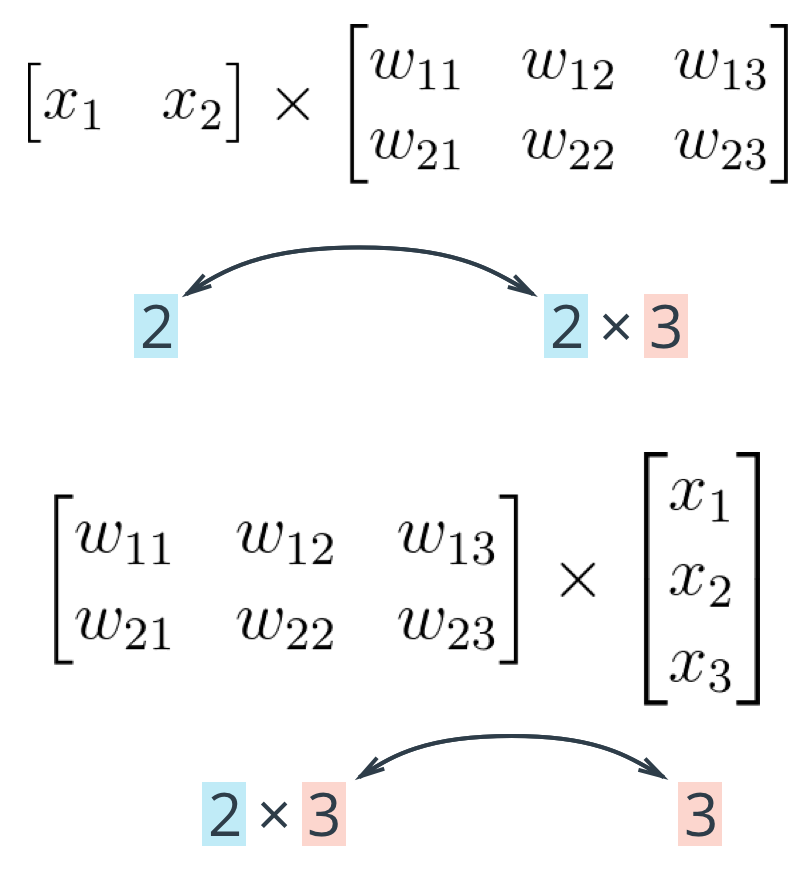
\includegraphics[width=0.5\linewidth]{img//intro//matrix-mult-3.png}

The rule is that if you're multiplying an array from the left, the array must have the same number of elements as there are rows in the matrix. And if you're multiplying the \textit{matrix} from the left, the number of columns in the matrix must equal the number of elements in the array on the right.

\paragraph{Making a column vector}

You see above that sometimes you'll want a column vector, even though by default NumPy arrays work like row vectors. It's possible to get the transpose of an array like so \lstinline{arr.T}, but for a 1D array, the transpose will return a row vector. Instead, use \lstinline{arr[:, None]} to create a column vector:

\begin{lstlisting}
print(features)
> array([ 0.49671415, -0.1382643 ,  0.64768854])

print(features.T)
> array([ 0.49671415, -0.1382643 ,  0.64768854])

print(features[:, None])
> array([[ 0.49671415],
       [-0.1382643 ],
       [ 0.64768854]])
\end{lstlisting}

Alternatively, you can create arrays with two dimensions. Then, you can use \lstinline{arr.T} to get the column vector.

\begin{lstlisting}
np.array(features, ndmin=2)
> array([[ 0.49671415, -0.1382643 ,  0.64768854]])

np.array(features, ndmin=2).T
> array([[ 0.49671415],
       [-0.1382643 ],
       [ 0.64768854]])
\end{lstlisting}

I personally prefer keeping all vectors as 1D arrays, it just works better in my head.

\subsubsection{Programming quiz}

Below, you'll implement a forward pass through a 4x3x2 network, with sigmoid activation functions for both layers.

Things to do:

\begin{itemize}
    \item Calculate the input to the hidden layer.
    \item Calculate the hidden layer output.
    \item Calculate the input to the output layer.
    \item Calculate the output of the network.
\end{itemize}

See notebook \verb|multilayer perceptrons.ipynb|

\subsubsection{Solution: Multilayer Perceptrons}

\begin{lstlisting}
import numpy as np

def sigmoid(x):
    """
    Calculate sigmoid
    """
    return 1/(1+np.exp(-x))

def forward_pass(x, weights_input_to_hidden, weights_hidden_to_output):
    """
    Make a forward pass through the network
    """
    # TODO: Calculate the input to the hidden layer.
    # Replace None with appropriate code
    hidden_layer_in = np.dot(x, weights_input_to_hidden)
    
    # TODO: Calculate the hidden layer output.
    # Replace None with appropriate code
    hidden_layer_out = sigmoid(hidden_layer_in)
    
    print('Hidden-layer Output:')
    print(hidden_layer_out)
    
    # TODO: Calculate the input to the output layer.
    # Replace None with appropriate code
    output_layer_in = np.dot(hidden_layer_out, weights_hidden_to_output)
    
    # TODO: Calculate the output of the network.
    # Replace None with approprite code
    output_layer_out = sigmoid(output_layer_in)
    
    print('Output-layer Output:')
    print(output_layer_out)
    
    return hidden_layer_out, output_layer_out

# Network size
N_input = 4
N_hidden = 3
N_output = 2

# Make some fake data
np.random.seed(42)
x = np.random.randn(N_input)
weights_input_to_hidden = np.random.normal(0, scale=0.1, size=(N_input, N_hidden))
weights_hidden_to_output = np.random.normal(0, scale=0.1, size=(N_hidden, N_output))

# Run forward_pass with fake data
hidden_layer_out, output_layer_out = forward_pass(x, weights_input_to_hidden, weights_hidden_to_output)
\end{lstlisting}

\section{Backpropagation}

Udacity video can be found on \href{https://www.youtube.com/watch?v=MZL97-2joxQ&t=22s&ab_channel=Udacity}{Youtube}. \newline

Now we've come to the problem of how to make a multilayer neural network \textit{learn}. Before, we saw how to update weights with gradient descent. The backpropagation algorithm is just an extension of that, using the chain rule to find the error with the respect to the weights connecting the input layer to the hidden layer (for a two layer network). \newline

To update the weights to hidden layers using gradient descent, you need to know how much error each of the hidden units contributed to the final output. Since the output of a layer is determined by the weights between layers, the error resulting from units is scaled by the weights going forward through the network. Since we know the error at the output, we can use the weights to work backwards to hidden layers.

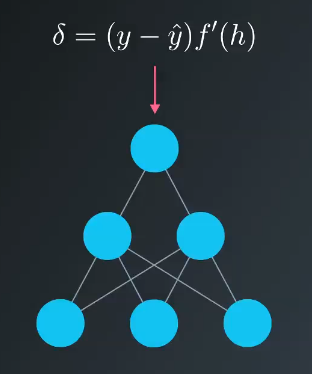
\includegraphics[width=0.5\linewidth]{img//intro/backpropagation-2.png}

The error for hidden units is proportional to the error in the output layer times the weight between the units. This is intuitive because the units with a stronger connection to the output node are going to contribute more error to the final output.

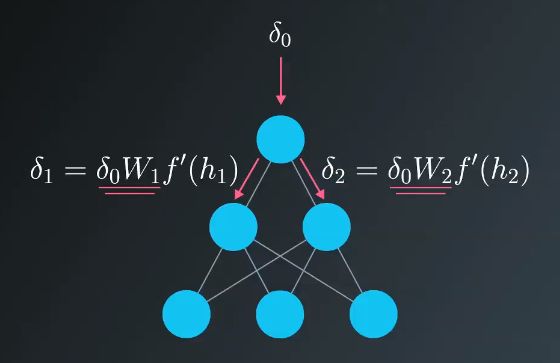
\includegraphics[width=0.5\linewidth]{img//intro/backpropagation-3.png}

Instead of propagating the inputs forward, we are propagating the error backwards through the network. Hence, you can view this process as flipping the network over and using the error as the input. 

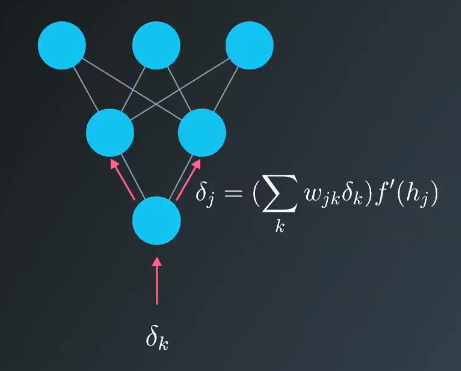
\includegraphics[width=0.5\linewidth]{img//intro/backpropagation-4.png}

The process is the same if there are more layers; you just keep backpropagating the error to the additional layers, as required.

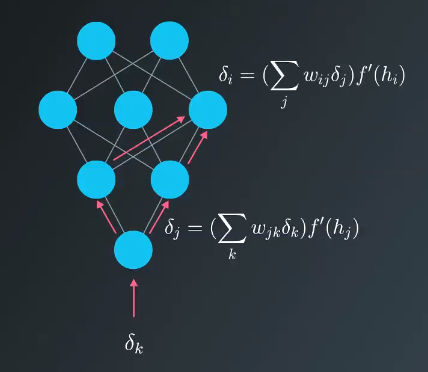
\includegraphics[width=0.5\linewidth]{img//intro/backpropagation-5.png}

\subsection{Mathematics of Backpropagation}

For example, in the output layer, you have errors \(\delta_k^o\) attributed to each output unit \(k\). Then, the \textbf{error} attributed to hidden unit \(j\) is the output errors, scaled by the weights between the output and hidden layers (and the gradient): \[\delta_j^k = \sum W_{jk} \delta _k^o f'(h_j)\]

Then, the \textbf{gradient descent step} is the same as before, just with the new errors: \[\Delta w_{ij} = \eta \delta_j^h x_i\]

where \(w_{ij}\) are the weights between the inputs and hidden layer and \(x_{ij}\) are input unit values. This form holds for however many layers there are. The \textbf{weight steps} are equal to the step size times the output error of the layer times the values of the inputs to that layer \[\Delta w_{pq} = \eta \delta_{output} V_{in}\]

Here, you get the output error, \(\delta_{output}\), by propagating the errors backwards from higher layers. And the input values, \(V_{in}\) are the inputs to the layer, the hidden layer activations to the output unit for example.

\subsection{Working through an example}

Let's walk through the steps of calculating the weight updates for a simple two layer network. Suppose there are two input values, one hidden unit, and one output unit, with sigmoid activations on the hidden and output units. The following image depicts this network. (\textbf{Note:} the input values are shown as nodes at the bottom of the image, while the network's output value is shown as \(\hat{y}\) at the top. The inputs themselves do not count as a layer, which is why this is considered a two layer network.)

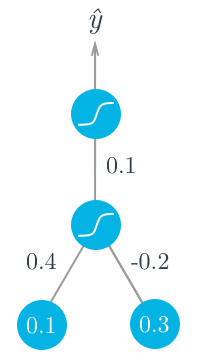
\includegraphics[width=0.5\linewidth]{img//intro//backprop-network.png}

Assume we're trying to fit some binary data and the target is \(y = 1\). We'll start with the forward pass, first calculating the input to the hidden unit \[h = \sum_i w_i x_i = (0.1 \cdot 0.4) - (0.2 \cdot 0.3) = -0.02\]
and the output of the hidden unit \[a = f(h) = sigmoid(-0.02) = 0.495\]

Using this as the input to the output unit, the output of the network is \[\hat{y} = f(W \cdot a) = sigmoid(0.1 \cdot 0.495) = 0.512\]

With the network output, we can start the backwards pass to calculate the weight updates for both layers. Using the fact that for the sigmoid function \[f'(W \cdot a) = f(W \cdot a)(1 - f(W \cdot a))\]
the error term for the output unit is \[\delta^o = (y-\hat{y})f'(W \cdot a) = (1 - 0.512) \cdot 0.512 \cdot (1-0.512) = 0.122\]

Now we need to calculate the error term for the hidden unit with backpropagation. Here we'll scale the error term from the output unit by the weight \(W\) connecting it to the hidden unit. For the hidden unit error term, \(\delta_j^h = \sum_k W_{jk} \delta_k^o f'(h_j)\), but since we have one hidden unit and one output unit, this is much simpler. \[\delta^h = W \delta^o f'(h) = 0.1 \cdot 0.122 \cdot 0.495 \cdot (1 - 0.495) = 0.003\]

Now that we have the errors, we can calculate the gradient descent steps. The hidden to output weight step is the learning rate, times the output unit error, times the hidden unit activation value. \[\Delta W = \eta \delta^O a = 0.5 \cdot 0.122 \cdot 0.495 = 0.0302\]

Then, for the input to hidden weights\(w_i\), t's the learning rate times the hidden unit error, times the input values. \[\Delta w_i = \eta \delta^h x_i = (0.5 \cdot 0.003 \cdot 0.1, 0.5 \cdot 0.003 \cdot 0.3) = (0.00015, 0.00045)\]
From this example, you can see one of the effects of using the sigmoid function for the activations. The maximum derivative of the sigmoid function is 0.25, so the errors in the output layer get reduced by at least 75\%, and errors in the hidden layer are scaled down by at least 93.75\%! You can see that if you have a lot of layers, using a sigmoid activation function will quickly reduce the weight steps to tiny values in layers near the input. This is known as the \textbf{vanishing gradient} problem. Later in the course you'll learn about other activation functions that perform better in this regard and are more commonly used in modern network architectures.

\subsection{Implementing in NumPy}

For the most part you have everything you need to implement backpropagation with NumPy.

However, previously we were only dealing with error terms from one unit. Now, in the weight update, we have to consider the error for \textit{each unit} in the hidden layer, \(\delta_j\): \[\Delta w_i = \eta \delta^h x_i\]
Firstly, there will likely be a different number of input and hidden units, so trying to multiply the errors and the inputs as row vectors will throw an error:

\begin{lstlisting}
hidden_error*inputs
---------------------------------------------------------------------------
ValueError                                Traceback (most recent call last)
<ipython-input-22-3b59121cb809> in <module>()
----> 1 hidden_error*x

ValueError: operands could not be broadcast together with shapes (3,) (6,) 
\end{lstlisting}

Also, \(w_{ij}\) is a matrix now, so the right side of the assignment must have the same shape as the left side. Luckily, NumPy takes care of this for us. If you multiply a row vector array with a column vector array, it will multiply the first element in the column by each element in the row vector and set that as the first row in a new 2D array. This continues for each element in the column vector, so you get a 2D array that has shape \lstinline{(len(column_vector), len(row_vector))}.

\begin{lstlisting}
hidden_error*inputs[:,None]
array([[ -8.24195994e-04,  -2.71771975e-04,   1.29713395e-03],
       [ -2.87777394e-04,  -9.48922722e-05,   4.52909055e-04],
       [  6.44605731e-04,   2.12553536e-04,  -1.01449168e-03],
       [  0.00000000e+00,   0.00000000e+00,  -0.00000000e+00],
       [  0.00000000e+00,   0.00000000e+00,  -0.00000000e+00],
       [  0.00000000e+00,   0.00000000e+00,  -0.00000000e+00]])
\end{lstlisting}

It turns out this is exactly how we want to calculate the weight update step. As before, if you have your inputs as a 2D array with one row, you can also do \lstinline{hidden_error*inputs.T}, but that won't work if \lstinline{inputs} is a 1D array.

\subsection{Backpropagation exercise}
Below, you'll implement the code to calculate one backpropagation update step for two sets of weights. I wrote the forward pass - your goal is to code the backward pass.

Things to do

\begin{itemize}
    \item Calculate the network's output error.
    \item Calculate the output layer's error term.
    \item Use backpropagation to calculate the hidden layer's error term.
    \item Calculate the change in weights (the delta weights) that result from propagating the errors back through the network.
\end{itemize}

\begin{lstlisting}
import numpy as np

def sigmoid(x):
    """
    Calculate sigmoid
    """
    return 1/(1+np.exp(-x))

def forward_pass(x, weights_input_to_hidden, weights_hidden_to_output):
    """
    Make a forward pass through the network
    """
    # Calculate the input to the hidden layer.
    hidden_layer_in = np.dot(x, weights_input_to_hidden)
    # Calculate the hidden layer output.
    hidden_layer_out = sigmoid(hidden_layer_in)

    # Calculate the input to the output layer.
    output_layer_in = np.dot(hidden_layer_out, weights_hidden_to_output)
    # Calculate the output of the network.
    output_layer_out = sigmoid(output_layer_in)

    return hidden_layer_out, output_layer_out

def backward_pass(x, target, learnrate, hidden_layer_out, \
                  output_layer_out, weights_hidden_to_output):
    """
    Make a backward pass through the network
    """
    # TODO: Calculate output error
    # Replace None with appropriate code
    error = target - output_layer_out
    
    # TODO: Calculate error term for output layer
    # Replace None with appropriate code
    output_error_term = error * output_layer_out * (1 - output_layer_out)

    # TODO: Calculate error term for hidden layer
    # Replace None with appropriate code
    hidden_error_term = np.dot(output_error_term, weights_hidden_to_output) * hidden_layer_out * (1 - hidden_layer_out)
    
    # TODO: Calculate change in weights for hidden layer to output layer
    # Replace None with appropriate code
    delta_w_h_o = learnrate * hidden_layer_out * output_error_term
    
    # TODO: Calculate change in weights for input layer to hidden layer
    # Replace None with appropriate code
    delta_w_i_h = learnrate * hidden_error_term * x[:, None]

    
    return delta_w_h_o, delta_w_i_h

# Create data to run through the network
x = np.array([0.5, 0.1, -0.2])
target = 0.6
learnrate = 0.5
weights_input_to_hidden = np.array([
    [0.5, -0.6],
    [0.1, -0.2],
    [0.1, 0.7]
])
weights_hidden_to_output = np.array([0.1, -0.3])

# Forward pass
hidden_layer_out, output_layer_out = forward_pass(
    x, weights_input_to_hidden, weights_hidden_to_output
)

# Backward pass
delta_w_h_o, delta_w_i_h = backward_pass(
    x, target, learnrate, hidden_layer_out, output_layer_out, \
    weights_hidden_to_output
)

print('Change in weights for hidden layer to output layer:')
print(delta_w_h_o)
print('Change in weights for input layer to hidden layer:')
print(delta_w_i_h)
\end{lstlisting}

\section{Implementing Backpropagation}

Now we've seen that the error term for the output layer is \[\delta_k = (y_k - \hat{y}_k) f'(a_k)\]
and the error term for the hidden layer is \[\delta_k = \sum \big[w_{jk} \delta_k \big] f'(h_j)\]

For now we'll only consider a simple network with one hidden layer and one output unit. Here's the general algorithm for updating the weights with backpropagation:
\begin{itemize}
    \item Set the weight steps for each layer to zero
    \begin{itemize}
        \item The input to hidden weights \(\Delta w_{ij} = 0\)
        \item The hidden to output weights  \(\Delta W_j = 0\)
    \end{itemize}
    \item For each record in the training data:
    \begin{itemize}
        \item Make a forward pass through the network, calculating the output \(\hat{y}\)
        \item Calculate the error gradient in the output unit, \(\delta^o = (y - \hat{y})f'(z)\) where \(z = \sum_j W_j a_j\), the input to the output unit.
        \item Propagate the errors to the hidden layer 
        \item Update the weight steps:
        \begin{itemize}
            \item \(\Delta W_j = \Delta W_j + \delta^o a_j\)
            \item \(\Delta w_{ij} = \Delta w_{ij} + \delta_j^h a_i\)
        \end{itemize}
    \end{itemize}
    \item Update the weights, where \(\eta\) is the learning rate and \(m\) is the number of records:
    \begin{itemize}
        \item \(W_j = W_j + \frac{\eta \Delta W_j}{m}\)
        \item \(w_{ij} = w_{ij} + \frac{\eta \Delta w_{ij}}{m}\)
    \end{itemize}
    \item Repeat for \(e\) epochs
\end{itemize}

\subsection{Backpropagation exercise}

Now you're going to implement the backprop algorithm for a network trained on the graduate school admission data. You should have everything you need from the previous exercises to complete this one.

Your goals here:

\begin{itemize}
    \item Implement the forward pass.
    \item Implement the backpropagation algorithm.
    \item Update the weights.
\end{itemize}


\begin{lstlisting}
import numpy as np
from data_prep import features, targets, features_test, targets_test

def sigmoid(x):
    """
    Calculate sigmoid
    """
    return 1 / (1 + np.exp(-x))

def forward_pass(x, weights_input_to_hidden, weights_hidden_to_output):
    """
    Make a forward pass through the network
    """
    # Calculate the input to the hidden layer.
    hidden_layer_in = np.dot(x, weights_input_to_hidden)
    # Calculate the hidden layer output.
    hidden_layer_out = sigmoid(hidden_layer_in)

    # Calculate the input to the output layer.
    output_layer_in = np.dot(hidden_layer_out, weights_hidden_to_output)
    # Calculate the output of the network.
    output_layer_out = sigmoid(output_layer_in)

    return hidden_layer_out, output_layer_out


def backward_pass(x, target, learnrate, hidden_layer_out,
                  output_layer_out, weights_hidden_to_output):
    """
    Make a backward pass through the network
    """
    # Calculate output error
    error = target - output_layer_out

    # Calculate error term for output layer
    output_error_term = error * output_layer_out * (1 - output_layer_out)

    # Calculate error term for hidden layer
    hidden_error_term = np.dot(output_error_term, weights_hidden_to_output) * \
                    hidden_layer_out * (1 - hidden_layer_out)

    # Calculate change in weights for hidden layer to output layer
    delta_w_h_o = learnrate * output_error_term * hidden_layer_out

    # Calculate change in weights for input layer to hidden layer
    delta_w_i_h = learnrate * hidden_error_term * x[:, None]

    return delta_w_h_o, delta_w_i_h

def update_weights(weights_input_to_hidden, weights_hidden_to_output, 
                   features, targets, learnrate):
    """
    Complete a single epoch of gradient descent and return updated weights
    """
    delta_w_i_h = np.zeros(weights_input_to_hidden.shape)
    delta_w_h_o = np.zeros(weights_hidden_to_output.shape)
    
    # Loop through all records, x is the input, y is the target
    for x, y in zip(features.values, targets):
        ## Forward pass ##
        
        # TODO: Calculate the output using the forward_pass function.
        # Replace None with appropriate code
        hidden_layer_out, output_layer_out = forward_pass(x, weights_input_to_hidden, weights_hidden_to_output)
        
        ## Backward pass ##
        
        # TODO: Calculate the change in weights using the backward_pass
        # function.
        # Replace None with appropriate code
        delta_w_h_o, delta_w_i_h = backward_pass(x, y, learnrate, hidden_layer_out,
                  output_layer_out, weights_hidden_to_output)

    n_records = features.shape[0]
    # TODO: Update weights  (don't forget division by n_records or number
    # of samples). Pay attention to the order of variables returned by
    # backward_pass
    # Replace 0 with appropriate code
    weights_input_to_hidden += delta_w_i_h / n_records
    weights_hidden_to_output += delta_w_h_o / n_records
    
    return weights_input_to_hidden, weights_hidden_to_output

def gradient_descent(features, targets, epochs=2000, learnrate=0.9):
    """
    Perform the complete gradient descent process on a given dataset
    """
    # Use to same seed to make debugging easier
    np.random.seed(11)
    
    # Initialize loss and weights
    last_loss = None
    n_features = features.shape[1]
    n_hidden = 2
    weights_input_hidden = np.random.normal(scale=1 / n_features ** .5,
                                        size=(n_features, n_hidden))
    weights_hidden_output = np.random.normal(scale=1 / n_features ** .5,
                                         size=n_hidden)

    # Repeatedly update the weights based on the number of epochs
    for e in range(epochs):
        weights_input_hidden, weights_hidden_output = update_weights(
            weights_input_hidden, weights_hidden_output, features,
            targets, learnrate
        )

        # Printing out the MSE on the training set every 10 epochs.
        # Initially this will print the same loss every time. When all of
        # the TODOs are complete, the MSE should decrease with each
        # printout
        if e % (epochs / 10) == 0:
            hidden_output = sigmoid(np.dot(features, weights_input_hidden))
            out = sigmoid(np.dot(hidden_output,
                                 weights_hidden_output))
            loss = np.mean((out - targets) ** 2)
            if last_loss and last_loss < loss:
                print("Train loss: ", loss, "  WARNING - Loss Increasing")
            else:
                print("Train loss: ", loss)
            last_loss = loss
            
    return weights_input_hidden, weights_hidden_output

def calculate_accuracy(features, targets, weights_input_hidden,
                       weights_hidden_output):
    """
    Given features, targets, and weights for both hidden and output
    layers, calculate the accuracy of predictions
    """
    hidden_out = sigmoid(np.dot(features, weights_input_hidden))
    output_out = sigmoid(np.dot(hidden_out, weights_hidden_output))
    predictions = output_out > 0.5
    accuracy = np.mean(predictions == targets)
    return accuracy

# Calculate accuracy on test data
weights_input_hidden, weights_hidden_output = gradient_descent(
    features, targets)
accuracy = calculate_accuracy(features_test, targets_test,
                              weights_input_hidden, weights_hidden_output)
print("Prediction accuracy: {:.3f}".format(accuracy))
\end{lstlisting}

\section{Glossary}

For your reference, here are all the new terms we introduced in this lesson:

\begin{itemize}
    \item An \textbf{error function} is simply a function that measures how far the current state is from the solution
    \item \textbf{Maximum likelihood}- a model that gives the existing labels in our historical data the highest probability
    \item \textbf{Cross-Entropy} is a way of measuring the difference between two distributions.
    \item A \textbf{perceptron} is a major building block of neural networks. Perceptrons are graphs that have nodes and edges.
    \item The \textbf{backpropagation} algorithm uses the chain rule to find the error with the respect to the weights connecting the input layer to the hidden layer (for a two-layer network).
\end{itemize}
PreviousNextGive Page Feedback
